\documentclass{article}

\usepackage[english]{babel}
\usepackage[letterpaper,top=2cm,bottom=2cm,left=3cm,right=3cm,marginparwidth=1.75cm]{geometry}
\setlength{\parindent}{0pt}

\usepackage{amsmath}
\usepackage{amsthm}
\usepackage{amssymb}
\usepackage{graphicx}
\usepackage{float}
\usepackage{listings}
\usepackage[colorlinks=true, allcolors=blue]{hyperref}
\usepackage{xcolor}

\lstset{
  basicstyle=\ttfamily\small,
  numbers=left,
  numberstyle=\tiny,
  stepnumber=1,
  numbersep=8pt,
  backgroundcolor=\color{gray!10},
  frame=single,
  rulecolor=\color{gray!60},
  tabsize=2,
  captionpos=b,
  breaklines=true,
  breakatwhitespace=true,
  showstringspaces=false,
  keywordstyle=\color{blue},
  commentstyle=\color{green!50!black},
  stringstyle=\color{orange},
}

\DeclareMathOperator{\argmax}{arg\,max}
\DeclareMathOperator{\conv}{conv}
\DeclareMathOperator{\sign}{sign}

\newcommand{\EE}{\mathbb{E}}
\newcommand{\PP}{\mathbb{P}}
\newcommand{\cD}{\mathcal{D}}
\newcommand{\cF}{\mathcal{F}}
\newcommand{\cG}{\mathcal{G}}
\newcommand{\cH}{\mathcal{H}}
\newcommand{\cU}{\mathcal{U}}
\newcommand{\one}{\mathbf{1}}

\title{DSC 291: Learning Theory Assignment 7}
\author{Tongle Shen}

\begin{document}
\maketitle

\section{Part A: Kernel Methods}

\subsection{Problem 1. Norm-Based Kernel Bound}

For a fixed sample $S=(x_1,\dots,x_n)$,
$$
\widehat{\mathfrak{R}}_S(\cH_{K,B})
=
\EE_\sigma \sup_{\|w\|\le B}
\frac1n \sum_{i=1}^n \sigma_i \langle w,\phi(x_i)\rangle.
$$
Pull the inner product inside:
$$
\widehat{\mathfrak{R}}_S(\cH_{K,B})
=
\frac1n \EE_\sigma \sup_{\|w\|\le B}
\left\langle
w,\sum_{i=1}^n \sigma_i \phi(x_i)
\right\rangle.
$$
By Cauchy--Schwarz, the supremum over $\|w\|\le B$ equals
$$
B\left\|\sum_{i=1}^n \sigma_i \phi(x_i)\right\|,
$$
so
$$
\widehat{\mathfrak{R}}_S(\cH_{K,B})
=
\frac{B}{n}
\EE_\sigma
\left\|
\sum_{i=1}^n \sigma_i \phi(x_i)
\right\|.
$$
Apply Jensen to $\sqrt{\cdot}$:
$$
\widehat{\mathfrak{R}}_S(\cH_{K,B})
\le
\frac{B}{n}
\sqrt{
\EE_\sigma
\left\|
\sum_{i=1}^n \sigma_i \phi(x_i)
\right\|^2
}.
$$
Expand the squared norm:
$$
\EE_\sigma
\left\|
\sum_{i=1}^n \sigma_i \phi(x_i)
\right\|^2
=
\EE_\sigma
\sum_{i,j=1}^n \sigma_i \sigma_j \langle \phi(x_i),\phi(x_j)\rangle.
$$
Since the Rademacher signs are independent and centered,
$$
\EE[\sigma_i\sigma_j]=0
\quad\text{for }i\ne j,
\qquad
\EE[\sigma_i^2]=1,
$$
so all cross terms vanish:
$$
\EE_\sigma
\left\|
\sum_{i=1}^n \sigma_i \phi(x_i)
\right\|^2
=
\sum_{i=1}^n \|\phi(x_i)\|^2
=
\sum_{i=1}^n K(x_i,x_i).
$$
Therefore
$$
\widehat{\mathfrak{R}}_S(\cH_{K,B})
\le
\frac{B}{n}\sqrt{\sum_{i=1}^n K(x_i,x_i)}.
$$

Now average over $S\sim \cD^n$:
$$
\mathfrak{R}_{\cD,n}(\cH_{K,B})
\le
\frac{B}{n}
\EE_S
\sqrt{\sum_{i=1}^n K(x_i,x_i)}.
$$
By Jensen again,
$$
\mathfrak{R}_{\cD,n}(\cH_{K,B})
\le
\frac{B}{n}
\sqrt{
\EE_S \sum_{i=1}^n K(x_i,x_i)
}
=
\frac{B}{n}
\sqrt{
n\,\EE[K(X,X)]
}.
$$
Hence
$$
\mathfrak{R}_{\cD,n}(\cH_{K,B})
\le
\frac{B\sqrt{\EE[K(X,X)]}}{\sqrt{n}}.
$$

\subsection{Problem 2. Representer Theorem}

Let
$$
V:=\operatorname{span}\{\phi(x_1),\dots,\phi(x_n)\}\subseteq \cU.
$$
Take any $w\in\cU$ and decompose it orthogonally as
$$
w=w_\parallel + w_\perp,
\qquad
w_\parallel \in V,
\qquad
w_\perp \perp V.
$$
Since every $\phi(x_i)\in V$,
$$
\langle w,\phi(x_i)\rangle
=
\langle w_\parallel,\phi(x_i)\rangle
+
\langle w_\perp,\phi(x_i)\rangle
=
\langle w_\parallel,\phi(x_i)\rangle.
$$
So the data-fit term in
$$
J(w)
=
\frac1n\sum_{i=1}^n \operatorname{loss}(\langle w,\phi(x_i)\rangle;y_i)
+
\lambda \|w\|^2
$$
depends only on $w_\parallel$.

For the regularizer,
$$
\|w\|^2
=
\|w_\parallel\|^2+\|w_\perp\|^2
\ge
\|w_\parallel\|^2.
$$
Hence
$$
J(w)\ge J(w_\parallel).
$$
Therefore any minimizer can be replaced by one lying in $V$. So whenever $J$ attains a minimum, some minimizer has the form
$$
w^\star = \sum_{j=1}^n \alpha_j \phi(x_j)
$$
for coefficients $\alpha\in\mathbb{R}^n$.

Now compute the prediction on $x_i$:
$$
\langle w^\star,\phi(x_i)\rangle
=
\sum_{j=1}^n \alpha_j \langle \phi(x_j),\phi(x_i)\rangle
=
\sum_{j=1}^n \alpha_j K(x_j,x_i)
=
(K_S \alpha)_i.
$$
Also
$$
\|w^\star\|^2
=
\left\langle
\sum_{i=1}^n \alpha_i \phi(x_i),
\sum_{j=1}^n \alpha_j \phi(x_j)
\right\rangle
=
\sum_{i,j=1}^n \alpha_i \alpha_j K(x_i,x_j)
=
\alpha^\top K_S \alpha.
$$
Thus the infinite-dimensional optimization problem is equivalent to
$$
\min_{\alpha\in\mathbb{R}^n}
\left[
\frac1n\sum_{i=1}^n \operatorname{loss}\bigl((K_S\alpha)_i;y_i\bigr)
+
\lambda \alpha^\top K_S \alpha
\right].
$$
All dependence on the sample enters only through the Gram matrix $K_S$.

\newpage
\section{\texorpdfstring{Part B: $\ell_1$ Rademacher Complexity}{Part B: l1 Rademacher Complexity}}

\subsection{Problem 1. Convex Hulls}

For any fixed realization of the signs $\sigma=(\sigma_1,\dots,\sigma_n)$, define
$$
c_f(\sigma)
:=
\frac1n \sum_{i=1}^n \sigma_i f(x_i).
$$
Then
$$
\sup_{h\in \conv(\cF)} \frac1n \sum_{i=1}^n \sigma_i h(x_i)
=
\sup_{\substack{a_f\ge 0\\ \sum_f a_f=1}}
\sum_{f\in\cF} a_f c_f(\sigma).
$$
The right-hand side is the maximum of a linear function over the simplex, so it is attained at an extreme point:
$$
\sup_{\substack{a_f\ge 0\\ \sum_f a_f=1}}
\sum_{f\in\cF} a_f c_f(\sigma)
=
\max_{f\in\cF} c_f(\sigma)
=
\sup_{f\in\cF} \frac1n\sum_{i=1}^n \sigma_i f(x_i).
$$
Taking expectation over $\sigma$ yields
$$
\widehat{\mathfrak{R}}_S(\conv(\cF))
=
\widehat{\mathfrak{R}}_S(\cF).
$$

\subsection{\texorpdfstring{Problem 2. $\ell_1$ Linear Predictors}{Problem 2. l1 Linear Predictors}}

Define the finite class
$$
\cF_0
=
\{0\}\cup \{x\mapsto B\phi_j(x):j\in[d]\}\cup \{x\mapsto -B\phi_j(x):j\in[d]\}.
$$
Every function in $\cF_0$ takes values in $[-BR,BR]$ because $\|\phi(x)\|_\infty\le R$.

Now let $h_w(x)=\langle w,\phi(x)\rangle$ with $\|w\|_1\le B$. Write
$$
h_w(x)
=
\sum_{j=1}^d w_j \phi_j(x)
=
\sum_{j=1}^d \frac{|w_j|}{B}\,\sign(w_j)\,B\phi_j(x).
$$
If $\|w\|_1<B$, add the missing weight
$$
1-\frac{\|w\|_1}{B}
$$
to the zero function. Hence $h_w\in \conv(\cF_0)$. Therefore
$$
\cH_B^1 \subseteq \conv(\cF_0).
$$
Using Problem 1,
$$
\widehat{\mathfrak{R}}_S(\cH_B^1)
\le
\widehat{\mathfrak{R}}_S(\conv(\cF_0))
=
\widehat{\mathfrak{R}}_S(\cF_0).
$$

Massart's finite-class lemma now gives
$$
\widehat{\mathfrak{R}}_S(\cF_0)
\le
BR \sqrt{\frac{2\log |\cF_0|}{n}}
\le
BR \sqrt{\frac{2\log(2d+1)}{n}}.
$$
So
$$
\widehat{\mathfrak{R}}_S(\cH_B^1)
\le
BR \sqrt{\frac{2\log(2d+1)}{n}}
=
O\!\left(
BR\sqrt{\frac{\log d}{n}}
\right).
$$
This is the desired logarithmic-in-dimension bound.

\subsection{\texorpdfstring{Problem 3. Comparison with Sparsity Bounds}{Problem 3. Comparison with Sparsity Bounds}}

Let $\ell(\widehat{y},y)$ be $G$-Lipschitz in $\widehat{y}$ and bounded in $[0,1]$. By contraction,
the Rademacher complexity of the loss class is at most
$$
G\,\widehat{\mathfrak{R}}_S(\cH_B^1).
$$
Using the Week 7 uniform-convergence theorem together with Problem 2, there is a universal constant $C$ such that, with probability at least $1-\delta$ over $S\sim \cD^n$, simultaneously for all $\|w\|_1\le B$,
$$
L^\ell_{\cD}(w)-L^\ell_S(w)
\le
C\left(
GBR\sqrt{\frac{\log(2d+1)}{n}}
+
\sqrt{\frac{\log(1/\delta)}{n}}
\right).
$$

\subsubsection{Comparison with the Sparse VC Bound}

The Week 4 sparsity bound says that for a $k$-sparse linear classifier,
$$
L^{0/1}_{\cD}(h)-L^{0/1}_S(h)
\le
C'
\sqrt{
\frac{k\log(ed/k)+\log(1/\delta)}{n}
}.
$$
The two guarantees measure different notions of complexity.
\begin{itemize}
\item In the sparsity bound, the complexity is the support size $k$.
\item In the $\ell_1$ Rademacher bound, the complexity is the norm budget $B$ together with the feature scale $R$, and the dimension enters only through $\log d$.
\end{itemize}

So the VC bound is \emph{support-sensitive}, while the Rademacher bound is \emph{scale-sensitive}. They are not interchangeable because they control different loss functionals.

The $\ell_1$ bound does not directly control $0/1$ error. To say anything about classification error, one needs an extra step: use a Lipschitz surrogate that upper-bounds or dominates $0/1$ loss, such as hinge loss or the ramp loss from Week 7, and then convert small surrogate risk into a classification statement.

Finally, the $\ell_1$ bound can be informative when sparsity is not. Consider the dense vector
$$
w=\left(\frac{B}{d},\dots,\frac{B}{d}\right),
$$
so $\|w\|_1=B$ but its support size is
$$
k=d.
$$
If $d\gg n$, then the sparsity bound becomes
$$
\Omega\!\left(\sqrt{\frac{d}{n}}\right),
$$
which is vacuous. By contrast, the $\ell_1$ bound is only
$$
O\!\left(
BR\sqrt{\frac{\log d}{n}}
\right),
$$
which can still be meaningful for moderate $B$.

\newpage
\section{\texorpdfstring{Part C: Normalized $\ell_1$ Margins and FixedBoost}{Part C: Normalized l1 Margins and FixedBoost}}

\subsection{Problem 1. Margin Generalization}

Fix $w\neq 0$ with empirical normalized margin
$$
\operatorname{margin}_S(w)
=
\min_i \frac{y_i f_w(x_i)}{\|w\|_1}
\ge
\gamma.
$$
Set
$$
u:=\frac{w}{\|w\|_1},
$$
so $\|u\|_1=1$ and
$$
y_i f_u(x_i)\ge \gamma
\qquad
\text{for every }i.
$$

Define the rescaled ramp loss
$$
\psi_\gamma(z)
:=
\min\{1,(1-z/\gamma)_+\}.
$$
It satisfies:
\begin{itemize}
\item $\one[z\le 0]\le \psi_\gamma(z)$ for all $z$,
\item $\psi_\gamma$ is $(1/\gamma)$-Lipschitz,
\item $\psi_\gamma(z)=0$ whenever $z\ge \gamma$.
\end{itemize}
Therefore
$$
\frac1n\sum_{i=1}^n \psi_\gamma(y_i f_u(x_i))=0.
$$

Now view $u$ as an $\ell_1$-bounded linear predictor over the feature map
$$
\Phi(x):=(g(x))_{g\in\cG}\in\{-1,+1\}^{|\cG|},
$$
so
$$
\|\Phi(x)\|_\infty=1.
$$
Apply the Part B.3 generalization-gap bound with
$$
B=1,\qquad R=1,\qquad G=1/\gamma,
$$
and dimension $|\cG|$. With probability at least $1-\delta$, uniformly over all $\|u\|_1\le 1$,
$$
L_{\cD}^{\psi_\gamma}(u)-L_S^{\psi_\gamma}(u)
\le
C\left(
\frac{1}{\gamma}\sqrt{\frac{\log(2|\cG|+1)}{n}}
+
\sqrt{\frac{\log(1/\delta)}{n}}
\right)
$$
for a universal constant $C$.

Since the empirical surrogate loss is zero,
$$
L_{\cD}^{\psi_\gamma}(u)
\le
C\left(
\frac{1}{\gamma}\sqrt{\frac{\log(2|\cG|+1)}{n}}
+
\sqrt{\frac{\log(1/\delta)}{n}}
\right).
$$
Because $\psi_\gamma$ upper-bounds $0/1$ loss and $\sign(f_u)=\sign(f_w)$,
$$
L_{\cD}^{0/1}(\sign f_w)
\le
L_{\cD}^{\psi_\gamma}(u).
$$
Hence, with probability at least $1-\delta$,
$$
L_{\cD}^{0/1}(\sign f_w)
\le
C\left(
\frac{1}{\gamma}\sqrt{\frac{\log(2|\cG|+1)}{n}}
+
\sqrt{\frac{\log(1/\delta)}{n}}
\right).
$$
Up to constants, this is the desired margin bound in terms of $|\cG|$, $n$, $\gamma$, and $\delta$.

\subsection{Problem 2. FixedBoost Implication}

The black-box theorem says that under the weak-learning condition
$$
\forall D\in\Delta_n,\ \exists g\in\cG
\quad
\text{with weighted error }
\le
\frac12-\frac{\gamma}{2},
$$
FixedBoost returns $w_T$ after
$$
T=O\!\left(\frac{\log n}{\gamma^4}\right)
$$
rounds such that
$$
\min_i y_i f_{w_T}(x_i)
\ge
\frac{\gamma}{2}\|w_T\|_1.
$$
Equivalently,
$$
\operatorname{margin}_S(w_T)\ge \frac{\gamma}{2}.
$$

Applying Problem 1 with margin parameter $\gamma/2$, we obtain that with probability at least $1-\delta$,
$$
L_{\cD}^{0/1}(\sign f_{w_T})
\le
C\left(
\frac{1}{\gamma}\sqrt{\frac{\log(2|\cG|+1)}{n}}
+
\sqrt{\frac{\log(1/\delta)}{n}}
\right)
$$
for another universal constant $C$.

So the classifier returned by FixedBoost generalizes at a rate controlled by the achieved normalized $\ell_1$ margin, not by the number of rounds directly. The round count only enters indirectly through the theorem that guarantees a margin of order $\gamma$.

\subsection{\texorpdfstring{Problem 3. Weak Learning and Normalized $\ell_1$ Margin}{Problem 3. Weak Learning and Normalized l1 Margin}}

Let $m:=|\cG|$ and write the sign matrix as
$$
A\in\{-1,+1\}^{n\times m},
\qquad
A_{ig}=y_i g(x_i).
$$

\subsubsection{Weak-Learning Edge}

For a distribution $D\in\Delta_n$ over the sample, the weighted error of $g$ is
$$
\sum_{i=1}^n D_i \one[g(x_i)\ne y_i]
=
\frac12-\frac12\sum_{i=1}^n D_i y_i g(x_i)
=
\frac12-\frac12 (D^\top A)_g.
$$
Therefore the edge of $g$ under $D$ is
$$
\frac12-\text{err}_D(g)
=
\frac12(D^\top A)_g.
$$
So the best weak-learning edge of the sample is
$$
\gamma_{\mathrm{weak}}
=
\frac12 \min_{D\in\Delta_n}\max_{g\in\cG}(D^\top A)_g.
$$

\subsubsection{Normalized Margin}

Because $\cG$ is symmetric, any negative coefficient on $g$ can be absorbed as a positive coefficient on $-g$. So when maximizing normalized $\ell_1$ margin, we may restrict without loss of generality to nonnegative coefficients whose sum is $1$. Thus
$$
\max_w \operatorname{margin}_S(w)
=
\max_{u\in\Delta_m} \min_{i\in[n]} (Au)_i.
$$
Now
$$
\min_{i\in[n]} (Au)_i
=
\min_{D\in\Delta_n} D^\top A u,
$$
because minimizing a linear function over the simplex picks out the smallest coordinate. Hence
$$
\max_w \operatorname{margin}_S(w)
=
\max_{u\in\Delta_m} \min_{D\in\Delta_n} D^\top A u.
$$

By von Neumann's minimax theorem,
$$
\max_{u\in\Delta_m} \min_{D\in\Delta_n} D^\top A u
=
\min_{D\in\Delta_n} \max_{u\in\Delta_m} D^\top A u.
$$
For fixed $D$, maximizing over the simplex $\Delta_m$ picks the largest coordinate:
$$
\max_{u\in\Delta_m} D^\top A u
=
\max_{g\in\cG} (D^\top A)_g.
$$
Therefore
$$
\max_w \operatorname{margin}_S(w)
=
\min_{D\in\Delta_n}\max_{g\in\cG}(D^\top A)_g.
$$
Comparing with the expression for $\gamma_{\mathrm{weak}}$, we obtain the exact relationship
$$
\max_w \operatorname{margin}_S(w)
=
2\gamma_{\mathrm{weak}}.
$$

\subsection{Problem 4. Connection to Homework 6}

Homework 6 gave a one-sided implication:
a particular sparse comparator $w^\star$ with large normalized $\ell_1$ margin forces every reweighting to admit a coordinate rule with nontrivial edge. The comparator there was a \emph{specific sparse witness}, and the final generalization step turned $T$ rounds of boosting into a $T$-sparse linear predictor, then used a sparse-VC argument on the activated support.

The present margin viewpoint refines both parts of that story.
\begin{itemize}
\item The comparator changes from one chosen sparse witness $w^\star$ to the \emph{best possible normalized $\ell_1$ margin} over all ensembles of base rules.
\item The weak-learning statement becomes exact: by Problem 3, the best weak edge is exactly half of the best normalized $\ell_1$ margin.
\item The generalization argument changes from a support-size VC bound to a norm-based Rademacher bound. The resulting complexity depends on
$$
\frac{1}{\gamma}\sqrt{\frac{\log |\cG|}{n}},
$$
not on the number of nonzero coordinates or the number of rounds directly.
\end{itemize}

So Week 7 replaces the coarse ``how many rules were used?'' viewpoint by the sharper ``what normalized $\ell_1$ margin was achieved?'' viewpoint.

\newpage
\section{\texorpdfstring{Part D: FixedBoost Margin Experiment}{Part D: FixedBoost Margin Experiment}}

\subsection{Problem 1. Implementation}

The implementation is in the relative path \verb|code/fixedboost_experiment.py|, and the numerical output is in \verb|code/fixedboost_summary.json|. I implemented FixedBoost directly on the sign matrix
$$
A_{ig}=y_i g(x_i)\in\{-1,+1\}.
$$
The loop differs from Homework 6's AdaBoost harness in three ways:
\begin{itemize}
\item the step size is fixed at $\eta=0.1$ instead of using the adaptive AdaBoost coefficient,
\item the algorithm works directly with the matrix $A$ rather than recomputing correlations from raw features and labels,
\item the tracked quantity of interest is the normalized empirical $\ell_1$ margin together with the LP optimum, rather than only training error or exponential loss.
\end{itemize}

Because the base class consists of signed coordinate predictors, the optimal normalized $\ell_1$ margin can be written as the linear program
$$
\max_{\rho,u}\ \rho
$$
subject to
$$
Au \ge \rho \one,
\qquad
u\ge 0,
\qquad
\sum_g u_g = 1.
$$
The simplex constraint is enough because the signed base class is symmetric, so negative coefficients can be folded into positive weights on negated predictors.

\subsection{Problem 2. Optimal-Margin Comparison}

I used two deterministic instances.

\subsubsection{Large-Margin Instance}

The easy instance is the majority-of-three sample:
$$
x\in\{-1,+1\}^3
$$
ranges over all $8$ Boolean patterns, and the label is
$$
y=\sign(x_1+x_2+x_3).
$$
The LP returns the exact optimal normalized margin
$$
\rho^\star_{\mathrm{easy}} = \frac13.
$$
FixedBoost reaches half of this value by round $3$, reaches $90\%$ of it by round $3$, and in fact hits the exact optimum at round $3$. By round $120$ the run ends exactly at
$$
\operatorname{margin}_S(w_{120})=\frac13.
$$

This large margin comes from the structure of $A$: the three informative coordinate columns can be averaged so that every row keeps signed score at least $1$ out of total $\ell_1$ mass $3$.

\subsubsection{Small-Margin Instance}

The hard instance reuses the Homework 6 sign-matrix construction with $m=3$, so the underlying Boolean dimension is
$$
d=2m+1=7.
$$
I take the $7$ sign vectors from that construction, label every example by $+1$, and repeat the rows with multiplicities
$$
q=(1,1,1,2,2,4,4).
$$
This yields a $15$-example sample whose signed-coordinate matrix is hard for weak learning.

For this instance the LP returns
$$
\rho^\star_{\mathrm{hard}} \approx 0.0303.
$$
FixedBoost reaches half of this optimum by round $114$, reaches $90\%$ of it by round $510$, and by round $1500$ attains
$$
\operatorname{margin}_S(w_{1500}) \approx 0.0293,
$$
leaving a gap of only about
$$
9.7\times 10^{-4}.
$$

This small optimum reflects the structure of $A$: there are reweightings under which every signed coordinate looks only barely better than random, so no convex combination can make every row strongly positive at once.

\begin{figure}[H]
  \centering
  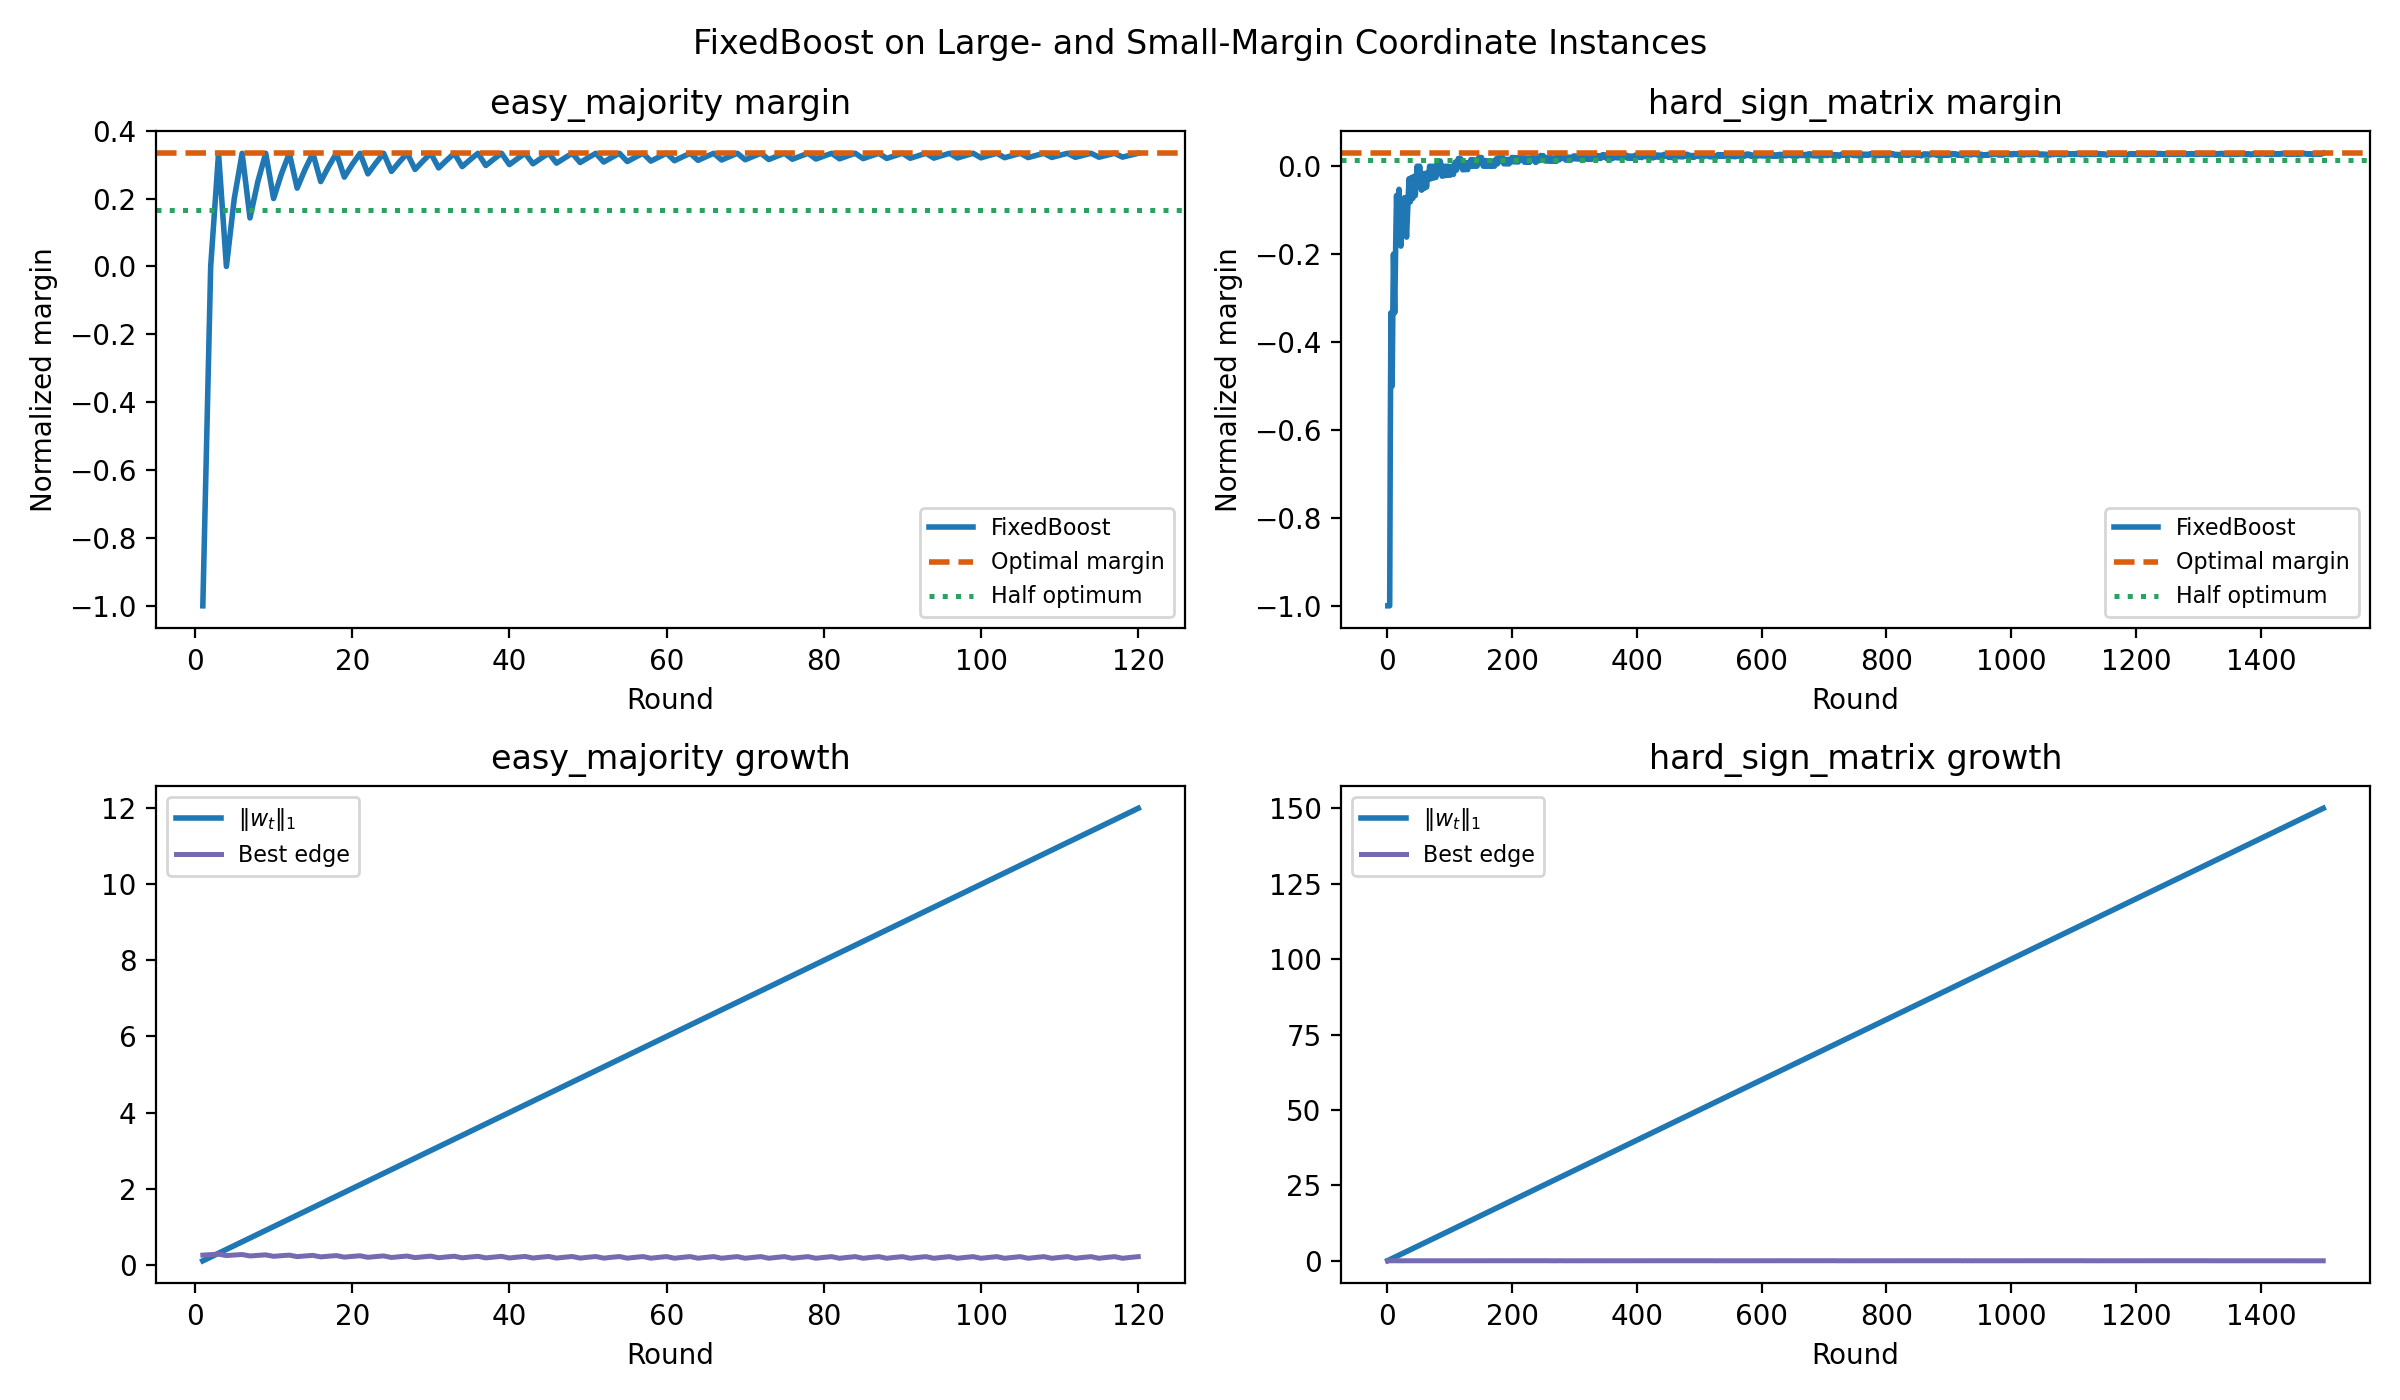
\includegraphics[width=1\linewidth]{figures/fixedboost_margin_comparison.png}
  \caption{FixedBoost normalized-margin trajectories and $\ell_1$ growth on the easy and hard instances.}
  \label{fig:hw7-fixedboost}
\end{figure}

\subsection{Problem 3. Interpretation}

Yes: on both instances, FixedBoost drives the normalized margin toward the LP optimum.

On the easy majority-of-three instance, convergence is essentially immediate: the optimum is exactly $1/3$, and the algorithm reaches it after three coordinate updates. The behavior is almost periodic after that because the same three informative columns keep reappearing.

On the hard sign-matrix instance, convergence is much slower but still clear. The optimum is only about $0.0303$, and the run gets to about $0.0293$ by round $1500$. The trajectory is therefore approaching the optimal value, but only after a long transient.

By Problem C.3, the theorem parameter $\gamma$ is exactly the optimal normalized margin $\rho^\star$. So the comparison with Part C.2 is especially revealing. The theorem-scale proxy
$$
\frac{\log n}{(\rho^\star)^4}
$$
is about
$$
168.4
$$
for the easy instance and about
$$
3.21\times 10^6
$$
for the hard instance. Empirically, however, the easy run reaches the optimum in $3$ rounds and the hard run reaches $90\%$ of optimum in $510$ rounds. So the theorem is qualitatively right but quantitatively very loose.

There are at least two reasons for the looseness.
\begin{itemize}
\item The theorem only guarantees a margin of order $\gamma/2$ after $O(\log n/\gamma^4)$ rounds; it does not try to predict when the iterates get close to the true optimum.
\item Problem C.3 is a minimax statement over \emph{all} reweightings $D$. The distributions actually visited by FixedBoost can be much friendlier than the adversarial worst-case distribution that defines $\rho^\star$.
\end{itemize}
So the experiment shows that the margin theorem is conservative: it gives a valid worst-case certificate, but it can be far slower and less precise than the dynamics observed on concrete samples.

\newpage
\section{Part E: Agent Skill Reflection}

\subsection{Problem 1. Existing Workflow}

I reused the existing repo workflow from \verb|AGENTS.md|: check that the \verb|ai4lt| Conda environment is active, use \verb|pdflatex| for builds, keep one companion statement file per homework, store code in \verb|hw7/code|, store plots in \verb|hw7/figures|, and keep long code out of the PDF by referencing the relative path instead.

\subsection{Problem 2. Skill Development}

I did not modify the local skill registry for this assignment, so the concrete skill I would add is a \verb|lt-margin-experiment| skill. It would automate four recurring tasks from this homework:
\begin{itemize}
\item build the sign matrix $A$ from labeled Boolean data,
\item solve the normalized-margin LP,
\item run a fixed-step boosting loop while logging margin and $\ell_1$ growth,
\item regenerate plots and a summary JSON so the LaTeX writeup can quote verified numbers.
\end{itemize}

\subsection{Problem 3. Verification}

The main coding-agent failure modes here are: mixing up the margin normalization by $\|w\|_1$, forgetting that symmetry lets negative coefficients be folded into positive weights on $-g$, solving the wrong LP, or reporting theorem quantities that do not match the implemented experiment.

I checked the assignment in several ways. For the math, I verified the minimax identities and the kernel/Rademacher derivations line by line against the exact problem statements and the Week 7 slides. For the code, I checked that the LP optimum on the easy instance is exactly $1/3$, which is analytically expected, and I confirmed that the hard instance produces a much smaller optimum. For the plots and reported claims, I regenerated \verb|code/fixedboost_summary.json| and the PNG figure from the script, then copied only those saved values into the final writeup. Finally, I rebuilt the PDF with \verb|pdflatex| to make sure the report and the repository artifacts are synchronized.

\end{document}
